\chapter[INTRODUÇÃO]{Introdução}

Este capítulo está organizado em seções, como ilustrado na figura 1, e apresenta uma visão geral do contexto onde a ferramenta desenvolvida está situada, bem como uma breve explanação acerca do \textit{framework} JADE, utilizado na investigação do Paradigma de Sistemas Multiagentes. Adicionalmente, são apresentados os objetivos que orientaram o desenvolvimento deste Trabalho de Conclusão de Curso. É apresentado ainda neste capítulo, o escopo final deste trabalho.

\begin{figure}[h!]
\centering
\label{f10}
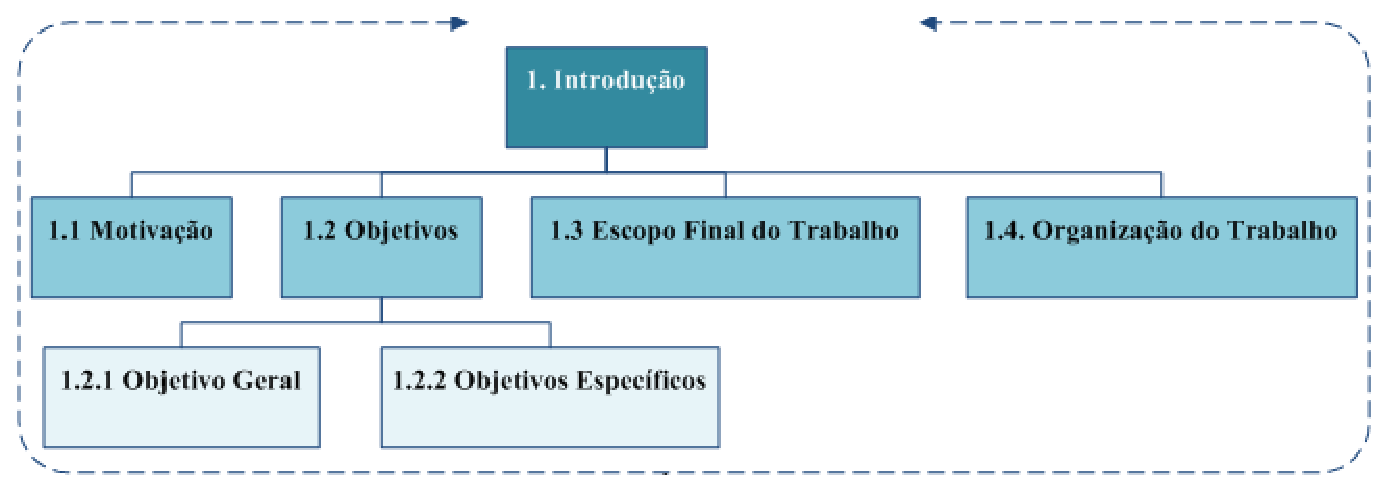
\includegraphics[width=1\textwidth]{figuras/cap1}
\caption{Organização do Capítulo}
\end{figure}
\FloatBarrier

\section{Motivação}


Bolsa de valores, de maneira geral, é um mercado organizado onde uma empresa pública ou privada abre seu capital para arrecadar fundos para fazer investimentos visando crescimento e maior lucro. Ao abrir o capital, a empresa disponibiliza uma quantidade de ações, que podem ser entendidas como pedaços da empresa. Esses, por sua vez, são vendidos para investidores, pessoas físicas/jurídicas ou estrangeiros. Essa empresa assume um compromisso de manter transparência com dados financeiros de interesse dos investidores e pode ser punida por um órgão regulador caso seja identificada alguma irregularidade.

Hoje no Brasil, existe apenas uma bolsa de valores, a Bolsa de Valores de São Paulo, que em 2014, só no mês de fevereiro, movimentou R\$ 131,54 bilhões com uma média de R\$ 6,57 bilhões por dia de pregão. Sendo que dessa movimentação, 50,42\% foi realizada por investidores estrangeiros, e apenas 13,73\% das movimentações vieram de investidores brasileiros pessoas físicas \cite{bovespa2014}.

Diante do exposto, percebe-se que o brasileiro não tem uma presença expressiva na bolsa de valores do país. Tal fato é comprovado por um estudo realizado pelo Instituto Rosenfield, encomendado pela BM\&FBovespa referente à educação financeira do brasileiro, o qual revelou que apenas 1\% da população investe em ações. Foram ouvidas pelo menos 2.000 pessoas das 15 maiores regiões metropolitanas brasileiras, abrangendo 100 municípios, de todas as classes sociais\cite{isabella2013}. O Estudo  publicado pela revista RI em 2013 também mostrou que:

\begin{citacao}
\begin{enumerate}
\item 40,8\% não fazem investimentos. Aplicam em poupança 44,4\% dos entrevistados, e 37\% deixam o dinheiro na conta corrente. Nem 5\% dos entrevistados investem em ao menos um dos demais investimentos, como imóveis, CDB (Certificado de Depósito Bancário), fundos DI (fundos de Depósito Interbancário), ações ou Tesouro Direto.
\item 52,6\% 	dos entrevistados preferem investimentos com baixo risco e baixa rentabilidade, confirmando o perfil conservador do brasileiro, e 65,6\% têm pouca propensão para investir em ações.
\item Os dois principais motivos para não investir em ações são a falta de conhecimento (para 43,5\% dos entrevistados) e o fato de não disponibilizar de dinheiro ao final do mês (para 21,3\% dos entrevistados).
\item Também há bastante desconhecimento sobre a diversificação dos investimentos. Como por exemplo, percebe-se que apenas 22\% dos entrevistados sabem que quando se investe em mais de um ativo, o risco de perder dinheiro diminui.\cite{isabella2013}

\end{enumerate}
\end{citacao}

Diante disto, é possível identificar um \textit{deficit} do cidadão brasileiro em relação aos conhecimentos necessários para investir. Investir na bolsa de valores requer alguns conhecimentos específicos que podem ser automatizados via Software. Um Software capaz de acompanhar e analisar determinados ativos de maneira autônoma, extraindo informações que auxiliem o cidadão a decidir como fazer seus próprios investimentos, de acordo com o seu perfil de investidor. Idealmente, seria como uma ferramenta guia, que mostraria ao cidadão outros tipos de investimentos além das aplicações em poupança. É exatamente essa necessidade que esse Trabalho de Conclusão de Curso procura atender.

Para desenvolver o Software proposto, foi abordado o Paradigma de Sistemas Multiagentes, no intuito de explorar o paradigma, aplicando-o ao contexto financeiro. Para isto foi escolhido o \textit{framework} JADE  \textit{(Java Agent Development Framework )}.

\begin{citacao}
O JADE é um framework completamente implementado na linguagem Java. Ele simplifica a implementação de sistemas multiagentes através de uma ponte que compila os agentes com as especificações FIPA e oferece suporte de ferramentas gráficas de acompanhamento e possibilidade de realizar atividades de debugging e deploy.  A plataforma de agentes é distribuída entre outros computadores (que não necessariamente possua o mesmo Sistema Operacional) e a configuração pode ser feita através de uma ferramenta remota. Um agente pode ser movido de um computador para outro em tempo de execução sempre que necessário. O JADE é completamente implementado na linguagem Java e requer pelo menos a versão 1.4 do JAVA, JRE ou  JDK, instalado. \cite{telecon2014}
\end{citacao}

Cada agente implementado nesta ferramenta possui um conjunto de comportamentos que define sua especialidade, comportamentos estes que podem ser abstraídos de investidores humanos existentes no contexto financeiro abordado neste estudo. Adicionalmente, cada agente tem a capacidade de ser autônomo o suficiente para utilizar este conjunto de comportamentos, até mesmo de forma colaborativa com outros agentes, visando alcançar determinados objetivos. No contexto abordado neste trabalho, um objetivo a ser alcançado pelos agentes seria a escolha, por exemplo, dos melhores investimentos alinhados ao perfil investidor do cidadão.

O propósito do Software, desenvolvido como Trabalho de Conclusão de Curso, é oferecer ao cidadão brasileiro uma ferramenta que o auxilie a realizar investimentos em bolsa de valores, de maneira simplificada e apoiada por estratégias financeiras. A ferramenta apresenta opções de investimentos de acordo com o perfil investidor do cidadão. Neste trabalho foram definidos três tipos de perfil investidor: (i) Corajoso, pessoa mais disposta a assumir riscos elevados; (ii) Moderado, pessoa que está entre o perfil Corajoso e Conservador; e (iii) Conservador, pessoa menos disposta a assumir riscos elevados.


\section{Objetivos}

Essa seção compreende os principais objetivos dessa pesquisa, organizados em: objetivo geral (Subseção 1.2.1) e objetivos específicos (Subseção 1.2.2).


\subsection {Objetivo Geral}

Construir uma Ferramenta de estratégia financeira apoiada por Sistemas Multiagentes Comportamentais, trabalhando a máquina de raciocínio dos agentes. Lembrando que a interface propriamente dita não é foco deste Trabalho de Conclusão de Curso, dado que os esforços  concentraram-se no raciocínio lógico dos agentes.


\subsection {Objetivos Específicos}

\begin{enumerate}
\item Abstrair a complexidade de cálculos financeiros comumente utilizados na Análise Técnica. Assim, essa complexidade não é sentida pelo usuário, deixando a mesma a cargo da ferramenta.
\item Explorar o Paradigma de Sistemas Multiagentes Comportamentais no contexto financeiro, implementando, por exemplo, comportamentos cíclicos e baseados em tempo.
\item Procurar facilitar a Reutilização de Software, em especial visando melhorar a manutenibilidade da ferramenta bem como sua extensibilidade em trabalhos futuros.
\item Procurar reduzir o acoplamento e aumentar a coesão, apoiando-se em boas práticas da Orientação a Objetos.
\end{enumerate}

\section{Escopo Final do Trabalho}

Ao conduzir o Trabalho de Conclusão de Curso, percebeu-se que o escopo final de trabalho compreende: (i) todo um estudo quanto ao paradigma de Sistemas Multiagentes aplicável ao Mercado de Bolsa de Valores, o qual orientou-se pela modalidade de pesquisa exploratória. Nesse caso, desenvolveu-se uma prova de conceito para embasar as decisões preliminares desse trabalho, e (ii) desenvolvimento propriamente dito da Ferramenta de Estratégia Financeira apoiada por Sistemas Multiagentes Comportamentais bem como a análise qualitativa dessa ferramenta quanto à qualidade do código obtido e as impressões coletadas junto aos potenciais usuários. 

Em resumo, o trabalho permitiu estudar uma abordagem emergente, desenvolver um produto de Software, e realizar ciclos evolutivos de teste e refinamento desse produto de Software com base nos resultados obtidos. Resultados esses oriundos da aplicação de pesquisa-ação \cite{rocha2012} (uma modalidade de pesquisa de natureza qualitativa). Esses aspectos serão principalmente retomados e acordados em detalhes nos capítulos Metodologia, Ferramenta Financeira e Resultados.

\section{Organização do Trabalho}

Este TCC está organizado em Capítulos. No \textbf{Capitulo 2}, concentra-se o referencial teórico, este organizado em Contexto Financeiro, com uma breve explanação sobre o mercado abordado, bem como em Engenharia de Software, com uma explanação do Paradigma de Sistemas Multiagentes. No \textbf{Capitulo 3}, concentra-se o suporte tecnológico deste TCC, este dividido em Contexto Financeiro, com uma exposição de alguns tipos de ferramentas de Software comumente encontradas no mercado para apoiar atividades de analises técnicas, bem como em Engenharia de Software, com a apresentação dos recursos utilizados neste TCC. No \textbf{Capitulo 4}, concentra-se a metodologia adotada. No \textbf{Capitulo 5}, concentra-se a descrição da ferramenta desenvolvida. No \textbf{Capitulo 6}, são apresentados os resultados obtidos. No \textbf{Capitulo 7}, são apresentadas as considerações finais desse estudo.




